% CRE-MI Methods Group journal club: Prevalent new-user cohort design 
% (c) 2021 Malcolm Gillies <malcolm.gillies@unsw.edu.au>
% https://github.com/mbg-unsw/pnuc
%
% This work is licensed under a
% Creative Commons Attribution-NonCommercial-ShareAlike 4.0
% International Licence
\documentclass[aspectratio=169,12pt]{beamer} % XXXX fix AR here
\usepackage[latin1]{inputenc}
\usepackage[T1]{fontenc}
\usepackage{textcomp}
\usefonttheme{serif} % need this with Charter font
\usetheme{Berlin}  % using default now
\usecolortheme{beaver}  % using default now
\usepackage[libertine]{libertine} % not using osf (old-style figures)
\usepackage[scale=0.9]{tgheros} % scale to match libertine
\usepackage[varqu,varl]{inconsolata}
\usepackage[libertine]{newtxmath}
\usepackage{graphicx}
\usepackage{tikz}
\usetikzlibrary{shadows}
\usepackage{tikzpagenodes}
\usepackage[round]{natbib}
\usepackage{gitinfo2}

\renewcommand{\gitMark}{\color{gray}\texttt{\tiny\gitBranch\,@\,\gitAbbrevHash\,\gitAuthorDate}}

\setbeamertemplate{navigation symbols}{} % remove navigation symbols
\setbeamercolor*{item}{fg=darkred}

\title{CRE-MI Methods Group journal club: Prevalent new-user cohort design}
\author{Malcolm Gillies}
\date{1 July 2021}
\usebackgroundtemplate{%
\begin{tikzpicture}[remember picture,overlay]
    \node[anchor=south west,scale=1,rotate=90] at ([shift={(0cm,0cm)}]current page marginpar area.south east) {\gitMark};
\end{tikzpicture}%
}

\newif\ifsidebartheme
\sidebarthemefalse

\newdimen\contentheight
\newdimen\contentwidth
\newdimen\contentleft
\newdimen\contentbottom
\makeatletter
\newcommand*{\calculatespace}{%
    \contentheight=\paperheight%
    \ifx\beamer@frametitle\@empty%
        \setbox\@tempboxa=\box\voidb@x%
      \else%
        \setbox\@tempboxa=\vbox{%
          \vbox{}%
          {\parskip0pt\usebeamertemplate***{frametitle}}%
        }%
        \ifsidebartheme%
          \advance\contentheight by-1em%
        \fi%
      \fi%
    \advance\contentheight by-\ht\@tempboxa%
    \advance\contentheight by-\dp\@tempboxa%
    \advance\contentheight by-\beamer@frametopskip%
    \ifbeamer@plainframe%
    \contentbottom=0pt%
    \else%
    \advance\contentheight by-\headheight%
    \advance\contentheight by\headdp%
    \advance\contentheight by-\footheight%
    \advance\contentheight by4pt%
    \contentbottom=\footheight%
    \advance\contentbottom by-4pt%
    \fi%
    \contentwidth=\paperwidth%
    \ifbeamer@plainframe%
    \contentleft=0pt%
    \else%
    \advance\contentwidth by-\beamer@rightsidebar%
    \advance\contentwidth by-\beamer@leftsidebar\relax%
    \contentleft=\beamer@leftsidebar%
    \fi%
}
\makeatother

\begin{document}

{
%\usebackgroundtemplate{}
\begin{frame}
\titlepage
\end{frame}
}

\begin{frame}{Today's paper}
\calculatespace%
\begin{columns}
\begin{column}{0.20\contentwidth}
\begin{tikzpicture}
  \node[drop shadow={shadow xshift=.8ex,shadow yshift=-.8ex},fill=white,draw] at (0,0) {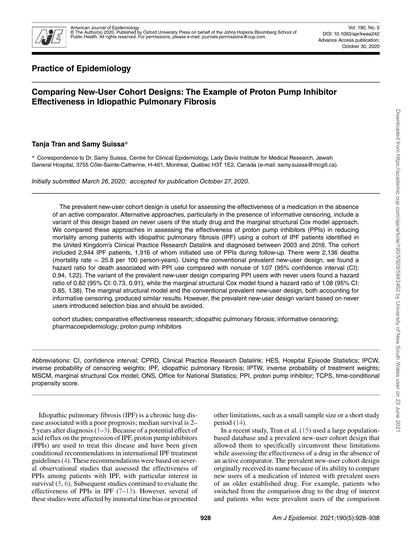
\includegraphics[width=\textwidth]{ref/suissa-pages-01_sm.jpg}};
\end{tikzpicture}
\end{column}
\begin{column}{0.70\contentwidth}
	\begin{itemize}
		\item T.~Tran and S.~Suissa. \textbf{Comparing {New}-{User} {Cohort} {Designs}: {The} {Example} of {Proton} {Pump} {Inhibitor} {Effectiveness} in {Idiopathic} {Pulmonary} {Fibrosis}.} \emph{American Journal of Epidemiology}, 190\penalty0 (5):\penalty0 928--938, May 2021. doi:10.1093/aje/kwaa242.
\nocite{tran_comparing_2021}
	\end{itemize}
\end{column}
\end{columns}
\end{frame}

% Introduce paper
% Introduce PNUC

\begin{frame}{Talk outline}
    \begin{itemize}
	\item Paper background
	\item Prevalent new-user cohort method in detail
	\item Adjusting for informative censoring
	\item Results
	\item What does the PNUC method estimate?
	\item Loose ends
    \end{itemize}
\end{frame}

\begin{frame}{Introduction}
    \begin{itemize}
	\item Question: Are PPIs efficacious in idiopathic pulmonary fibrosis?
	\item Contention: Effects seen in earlier studies are due to bias
	\item Data: UK linked GP and hospital data (CPRD-GOLD/HES/ONS), $n=2944$
	\item Outcomes: All-cause mortality, respiratory death, hospitalisation
	\item Covariates: Demographics, comorbidity, medicines (all time-varying)
    \end{itemize}
\end{frame}

\begin{frame}{Idiopathic Pulmonary Fibrosis (IPF)}
    \begin{itemize}
        \item Progressive scarring of the lungs, cause unknown
	\item Average life expectancy after diagnosis about four years
	\item Pirfenidone (2008) and nintedanib (2014) slow progression
	\item Proton pump inhibitors also guideline recommended (weak evidence)
    \end{itemize}
\end{frame}

\begin{frame}{Review: Active comparator new-user cohort design}
    \begin{itemize}
	\item Confounding by indication (inactive comparator)
	\item Healthy adherer bias (prevalent users)
    \end{itemize}
\end{frame}

\begin{frame}{Why \emph{prevalent} new-user?}
    \begin{itemize}
	\item Increase sample size if few treatment-naive patients
	\item Better external validity e.g. disease progression
	\item Key feature: conditioning on length of exposure
    \end{itemize}
\end{frame}

\begin{frame}{Prevalent new-user cohort design step by step}
    \begin{enumerate}
	\item Defining the base cohort
	\item Forming exposure sets
	\item Estimating the propensity score
	\item Matching and forming the analysis cohort
	\item Estimating the causal effect
    \end{enumerate}
\end{frame}

\begin{frame}{Defining exposure sets and estimating the propensity score}
    \calculatespace%
    \begin{center}
	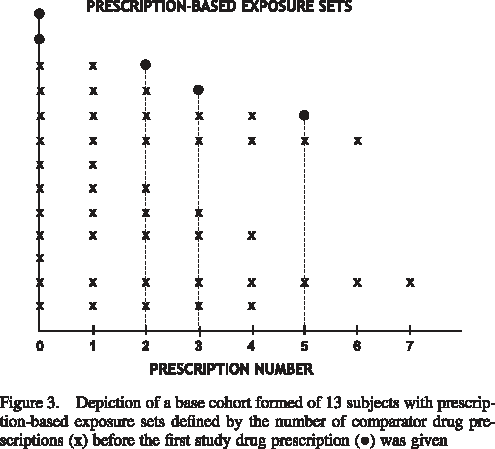
\includegraphics[height=0.85\contentheight]{ref/suimoodell-fig3.pdf}
    \end{center}
\flushright{\small{\citet{suissa_prevalent_2017}}}

\end{frame}

\begin{frame}{Matching}
    \calculatespace%
    \begin{center}
	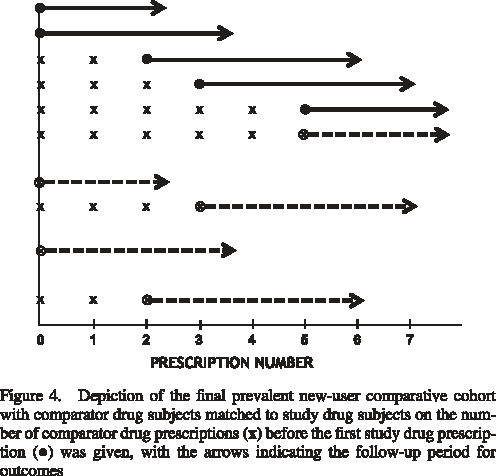
\includegraphics[height=0.85\contentheight]{ref/suimoodell-fig4.pdf}
    \end{center}
\flushright{\small{\citet{suissa_prevalent_2017}}}
\end{frame}

\begin{frame}{Informative censoring}
    \begin{itemize}
	\item In this study, ``prevalent user'' = IPF patient \emph{not}
	      treated with PPI
	\item Follow-up of prevalent users is censored if PPI treatment starts
	\item Starting PPI = patient is sicker (but still alive)
    \end{itemize}
\end{frame}

\begin{frame}{Adjusting for informative censoring}
    \begin{itemize}
	\item Option 1: Restriction
	\begin{itemize}
	    \item exclude PPI ever users from prevalent cohort
	\end{itemize}
	\item Option 2: Weighting
	\begin{itemize}
	    \item use inverse probability of censoring weights (IPCW)
	    \item estimate from logistic regression model (\emph{\`{a} la} propensity)
	\end{itemize}
    \end{itemize}
\end{frame}

\begin{frame}{Results 1}
    \calculatespace%
    \begin{center}
	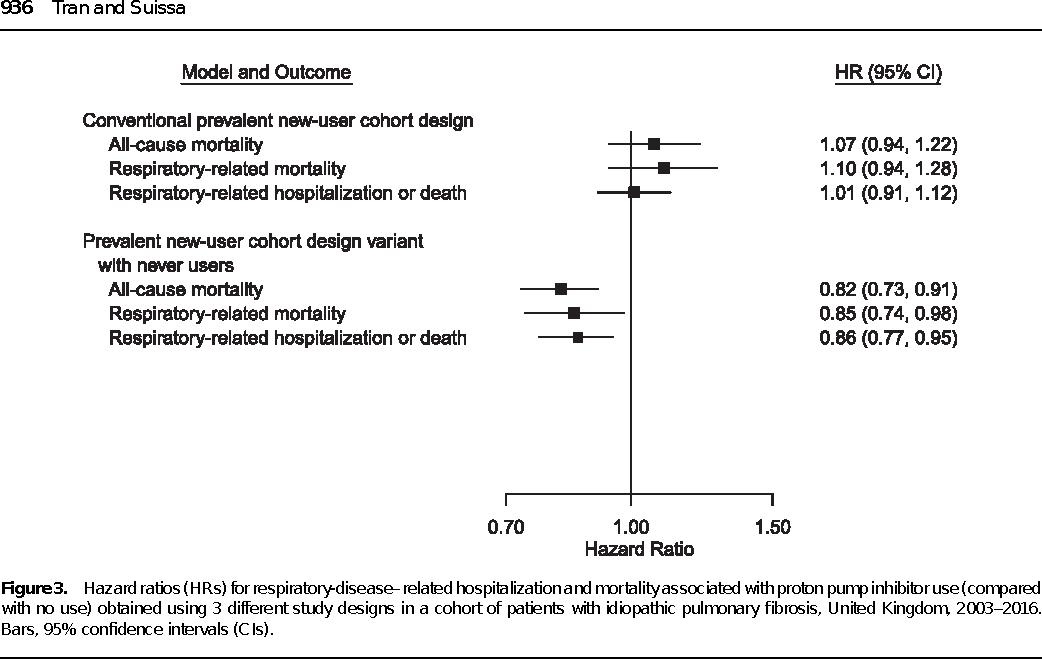
\includegraphics[height=0.90\contentheight]{ref/suissa-fig3-pnuc.pdf}
    \end{center}
\end{frame}

\begin{frame}{Marginal Structural Cox Model}
    \begin{itemize}
	\item All patients followed from IPF diagnosis
	\item Exposure and covariates assessed in each person-month
	\item Inverse probability of treatment weights (IPTW)
	\item Inverse probability of censoring weigts (IPCW)
	\item Estimation with weighted time-dependent Cox model
    \end{itemize}
\end{frame}

\begin{frame}{Results 2}
    \calculatespace%
    \begin{center}
	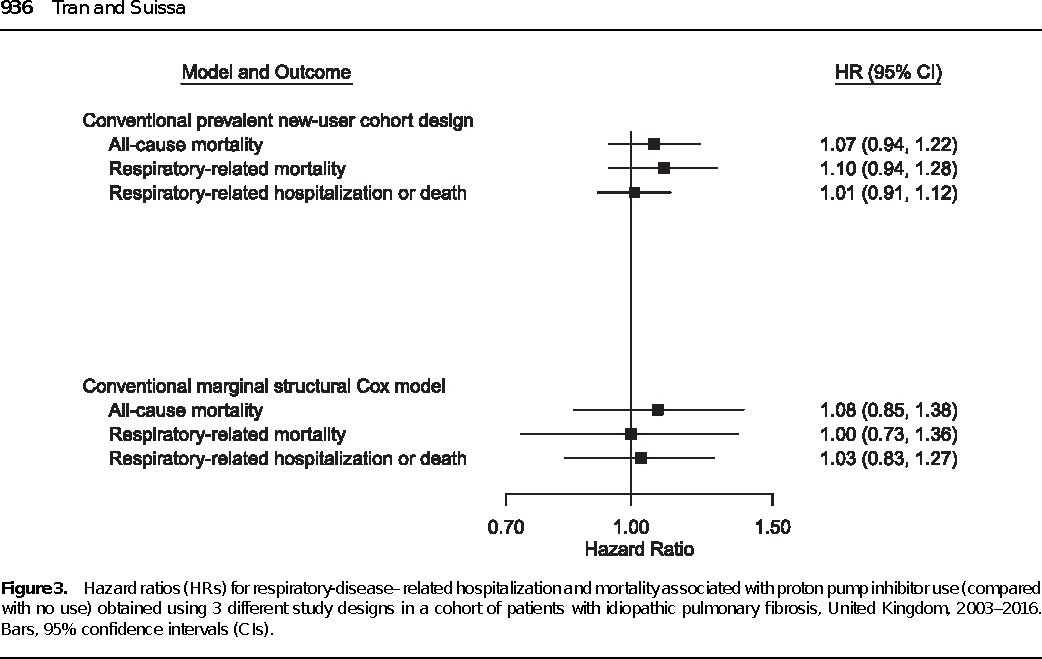
\includegraphics[height=0.90\contentheight]{ref/suissa-fig3-mscm.pdf}
    \end{center}
\end{frame}

\begin{frame}{Estimands}
    \calculatespace%
    \begin{center}
	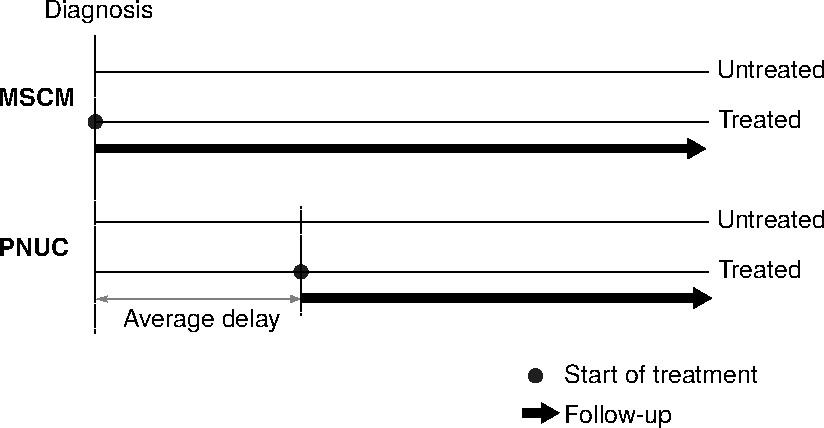
\includegraphics[height=0.95\contentheight]{ref/estimands.pdf}
    \end{center}
\end{frame}

\begin{frame}{Scenarios}
    \calculatespace%
	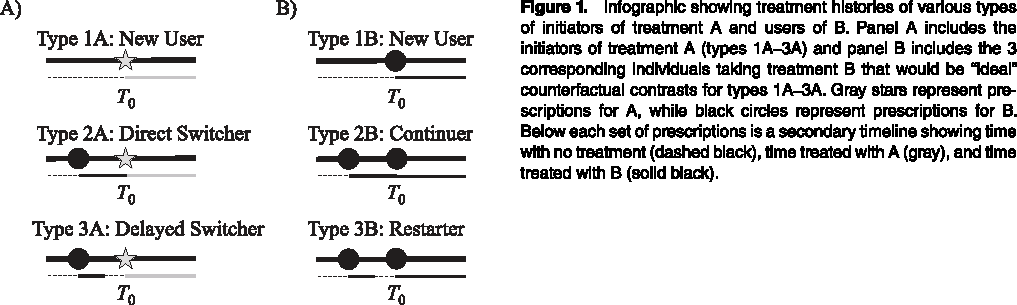
\includegraphics[width=0.85\contentwidth]{ref/webster-fig1.pdf}
\flushright{\small{\citet{webster-clark_initiator_2020}}}
\end{frame}

\begin{frame}{Loose ends}
    \begin{itemize}
	\item Sampling with/without replacement
	\item Conditioning on length of exposure vs entire history
	\item Positivity and matching
	\item Estimating the propensity score
	\item See also: \url{https://pharmacoepi.unc.edu/wp-content/uploads/sites/6788/2020/12/Webster-Clark_Michael_PNU.pdf}
    \end{itemize}
\end{frame}

%\usebackgroundtemplate{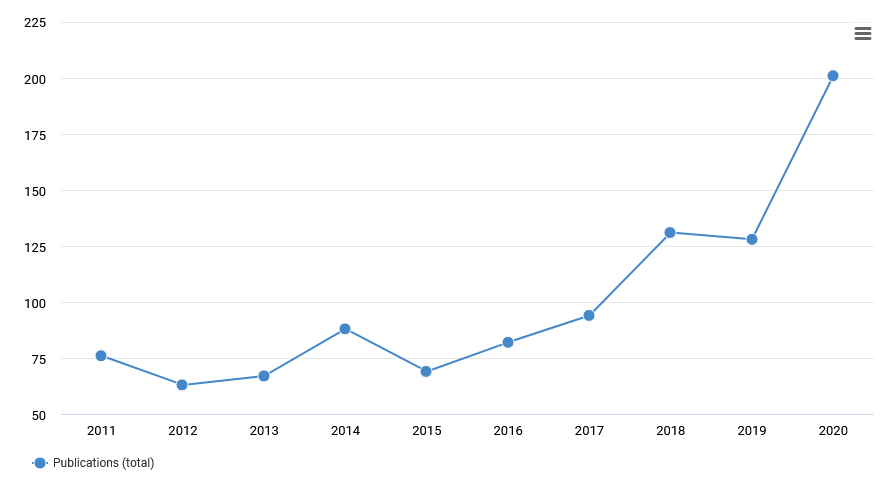
\includegraphics[width=\paperwidth]{ref/newey-west-cites.PNG}}
%\begin{frame}[plain,b]
%\begin{flushright}\texttt{https://app.dimensions.ai/}\end{flushright}
%\end{frame}
%\usebackgroundtemplate{}

\begin{frame}{Discussion}
    \begin{itemize}
	\item Have you used the prevalent new-user cohort design or the marginal structural Cox model approach? If so, please tell us about it.
    	\item Would you use either of these methods for your current research interests? What do you see as the barriers to using them?
    \end{itemize}
\end{frame}

\begin{frame}{Other business}
    \begin{itemize}
	\item Suggestions for articles or topics to discuss
	\item Volunteers to present
	\item Comments on format, timing, frequency and audience for the journal club
    \end{itemize}
\end{frame}

\begin{frame}{References}
        \tiny\bibliography{pnuc.bib}
        \bibliographystyle{abbrvnat}
\end{frame}

\end{document}
